\begin{figure}[h!]
\begin{center}
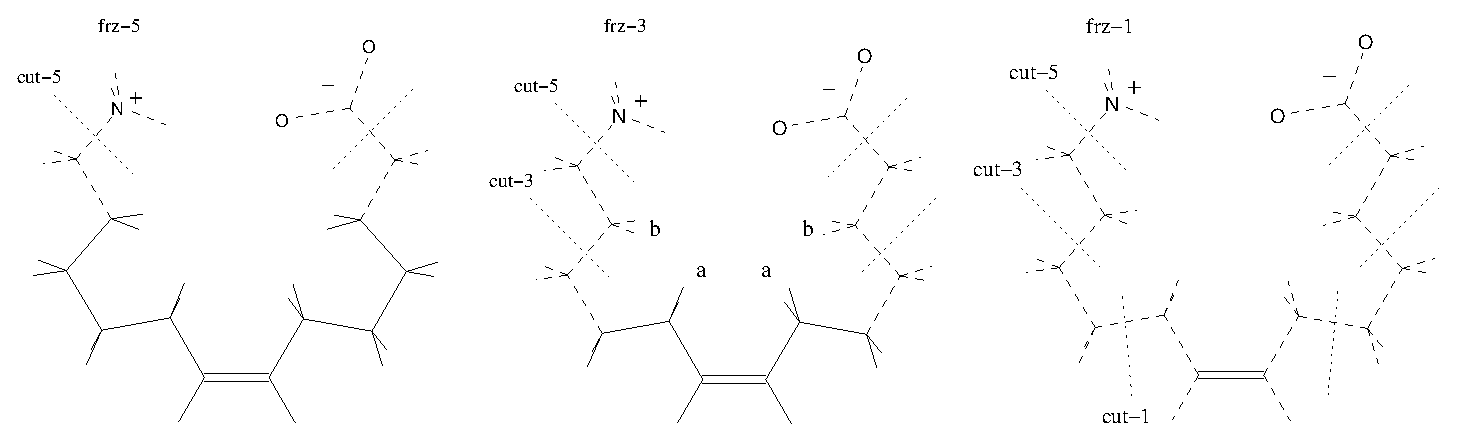
\includegraphics[width=12cm,keepaspectratio]{02_localization/images/7Z-frzcut-schema.eps}
\caption{\footnotesize (7Z)-13 ammoniotridec-7-enoate. Localized orbitals expressed on
atoms of the dashed line framework are frozen. Orbitals expressed on atoms
of the solid line framework are not frozen. Dotted lines depict the
cut seam. The cut is always performed on both chains, from ``cut-5'' (only
the charged groups are removed from the molecule, both left and right) to
``cut-1'' (maximal cut selection, only the central double bond and left and
right -CH$_{2}$- spacers are preserved). The ``a'' and ``b'' symbols in frz-3 picture
are labels for interesting hydrogen atoms. See text for details.  }
\label{fig:7Z-frzcut-schema}
\end{center}
\end{figure}
